\section[Midterm Solutions]{Midterm Solutions \iftoggle{showdates}{\small{\textit{2014-06-06}}}{}}
\subsection*{Question 1}\index{Bayes' Rule}
\begin{itemize}
  \item $T = $ positive test
  \item $\neg T = $ negative test
  \item $HIV = $ infected with HIV
  \item $\neg HIV = $ not infected with HIV
\end{itemize}

\index{Probability tree}
\begin{figure}[!ht]
  \centering
  \tikzstyle{level 1}=[level distance=1.5cm, sibling distance=6cm]
\tikzstyle{level 2}=[level distance=1.5cm, sibling distance=4.0cm]

\tikzstyle{bag} = [text width=4em, text centered]
\tikzstyle{end} = [circle, minimum width=3pt, fill, inner sep=0pt]

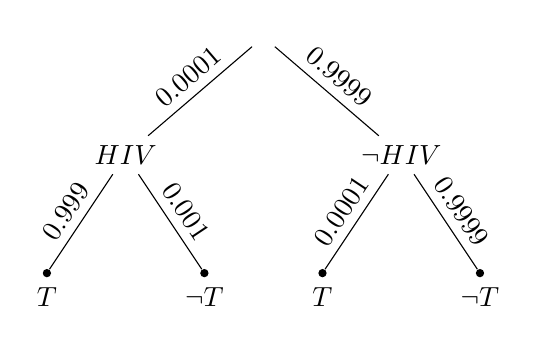
\begin{tikzpicture}[grow=down, sloped]
\node[bag] {}
    child {
        node[bag] {$HIV$}
        child {
            node[end, label=below: {$T$}] {}
            edge from parent
            node[above] {0.999}
        }
        child {
            node[end, label=below: {$\neg T$}] {}
            edge from parent
            node[above] {0.001}
        }
        edge from parent         
        node[above] {0.0001}
    }
    child {
        node[bag] {$\neg HIV$}
        child {
            node[end, label=below: {$T$}] {}
            edge from parent
            node[above] {0.0001}
        }
        child {
            node[end, label=below: {$\neg T$}] {}
            edge from parent
            node[above] {0.9999}
        }
        edge from parent         
        node[above] {0.9999}
    };
\end{tikzpicture}

  \caption{Probability tree}
  \label{fig:2014-06-06_mt1tree}
\end{figure}
We search for
\begin{align*}
P(HIV|T) = \frac{P(T|HIV)P(HIV)}{P(T)} = \frac{0.999\cdot 0.0001}{0.999 \cdot 0.0001+0.0001 \cdot 0.9999} = \frac{1110}{2221} < \frac{1}{2}
\end{align*}
The probability that A is infected with HIV is just below 0.5.



\subsection*{Question 2}
to be added...



\subsection*{Question 3}
The important clue for this question is that he has two win \textit{two consecutive} sets.

We can draw two simple probability trees\index{Probability tree}(figure \ref{fig:2014-06-06_mt3trees}) to calculate Elmer's chances. We use $f$ and $c$ (probability to win against father and champ, respectively) where $f > c$ denote the chances to win each set.
\begin{figure}[!ht]
  \centering
  \begin{subfigure}{.45\linewidth}
    \centering
    \input{images/MTexercise3tree1.tex}
    \caption{father-champ-father}
    \label{fig:2014-06-06_mt3tree1}
  \end{subfigure}
  \begin{subfigure}{.45\linewidth}
    \centering
    \tikzstyle{level 1}=[level distance=1.5cm, sibling distance=3.5cm]
\tikzstyle{level 2}=[level distance=1.5cm, sibling distance=2cm]
\tikzstyle{level 3}=[level distance=1.5cm, sibling distance=3cm]

\tikzstyle{bag} = [text width=4em, text centered]
\tikzstyle{end} = [circle, minimum width=3pt, fill, inner sep=0pt]

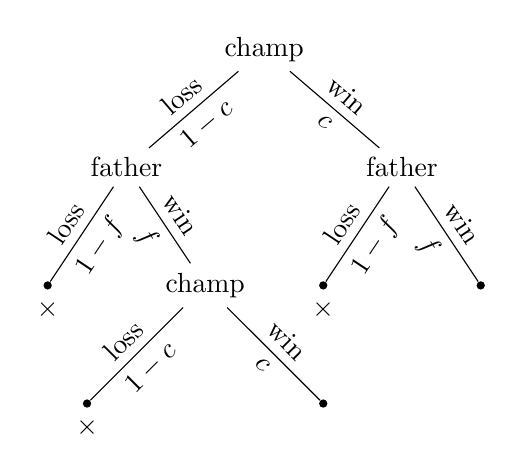
\begin{tikzpicture}[grow=down, sloped]
\node[bag] {champ}
    child {
        node[bag] {father}
        child {
            node[end, label=below: {$\times$}] {}
            edge from parent
            node[above] {loss}
            node[below] {$1-f$}
        }
        child {
            node[bag] {champ}
            child {
              node[end, label=below: {$\times$}] {}
              edge from parent
              node[above] {loss}
              node[below] {$1-c$}
            }
            child {
              node[end, label=below: {$\checkmark$}] {}
              edge from parent
              node[above] {win}
              node[below] {$c$}
            }
            edge from parent
            node[above] {win}
            node[below] {$f$}
        }
        edge from parent         
        node[above] {loss}
        node[below] {$1-c$}
    }
    child {
        node[bag] {father}
        child {
            node[end, label=below: {$\times$}] {}
            edge from parent
            node[above] {loss}
            node[below] {$1-f$}
        }
        child {
            node[end, label=below: {$\checkmark$}] {}
            edge from parent
            node[above] {win}
            node[below] {$f$}
        }
        edge from parent         
        node[above] {win}
        node[below] {$c$}
    };
\end{tikzpicture}

    \caption{champ-father-champ}
    \label{fig:2014-06-06_mt3tree2}
  \end{subfigure}
  \caption{Two possible choices}
  \label{fig:2014-06-06_mt3trees}
\end{figure}

We can see that in the first setup, father-champ-father, the probability to win two consecutive matches (those marked with $\checkmark$) is $fc+(1-f)cf=cf(2-f)$, and in the second setup accordingly: $cf+(1-c)fc=fc(2-c)$.

Since we know $f>c$ we can use this information to evaluate the odds\index{Odds}:
\begin{align*}
\frac{P(success|f-c-f)}{P(success|c-f-c)} = \frac{cf(2-f)}{cf(2-c)} = \frac{2-f}{2-c} < 1
\end{align*}
Since $\frac{2-f}{2-c} < 1$ the odds are in favor of the second setup: \textbf{champ-father-champ}.

This also makes sense intuitively because playing against the champ first gives a higher probability for a second chance in case the first match is lost. This of course only is valid since Elmer has to win two sets in a row.



\subsection*{Question 4}\index{Odds}
We can take advantage if we are able to set up a dutch book.
\begin{itemize}
	\item Bookie A: Real wins 1:3
  \item Bookie A: Real loses 4:1
	\item Bookie B: Real wins 1:5
  \item Bookie B: Real loses 6:1
\end{itemize}

As we can see Bookie B pays more for a win than we have to pay for a loss at Bookie A. We should be able to exploit this.

\begin{align*}
\frac{5}{1+5}+\frac{1}{1+4} = \frac{5}{6} + \frac{1}{5} = \frac{25}{30} + \frac{6}{30} = \frac{31}{30} > 1 \Rightarrow \text{A dutch book is possible}
\end{align*}

The expected value for win and loss when betting the scenario above are:
\begin{align*}
E(win)  &= 5x-y \\
E(loss) &= \frac{1}{4}y-x
\end{align*}
We can calculates for which interval we can make money:
\begin{align*}
E(win)  &= 5x-y           > 0 \Leftrightarrow 5x>y             \Leftrightarrow y < 5x \\
E(loss) &= \frac{1}{4}y-x > 0 \Leftrightarrow -x>-\frac{1}{4}y \Leftrightarrow 4x < y
\end{align*}
So we can take advantage by betting $x$ on win at B and $y$ on loss at A as long as $x$ and $y$ fulfill this inequality: $4x<y<5x$.



\subsection*{Question 5}
to be added...



\subsection*{Question 6}\index{Change of variable}
to be added...



\subsection*{Question 7}\index{Proper Scoring Rule}
To check if a proper scoring rule is given, we can check if it is minimal (since our function is a loss function) for $p=q$. So we take the $1^{st}$ derivative and set it to zero to see if $p=q$ holds. We have to check the second derivative to see whether we found a mini- or maximum.

\begin{align*}
                L(X,q) &= -Xq^2-(1-X)(1-q)^2 \\
\Leftrightarrow L(X,q) &= -Xq^2-(1-X)(1-2q+q^2) \\
\Leftrightarrow L(X,q) &= -Xq^2-1+2q-q^2+X-2Xq+Xq^2 \\
\Leftrightarrow L(X,q) &= -q^2+2q-2Xq+X-1 \\
\\
\text{Set }X&=p \\
L(p,q) &= -q^2+2q-2pq+p-1 \\
\frac{\partial L(p,q)}{\partial q} &= -2q+2-2p \\
\\
\text{Set }\frac{\partial L(p,q)}{\partial q}&=0 \\
-2q+2-2p &= 0\\
\Leftrightarrow 2-2p&=2q \\
\Leftrightarrow 1-p&=q \\
\\
\frac{\partial^2 L(p,q)}{\partial^2 q} &= -q \\
\frac{\partial^2 L(p,q)}{\partial^2 q} &< 0
\end{align*}
The $1^{st}$ derivative has an extreme value at $1-p=q$, however since this is a maximum ($2^{nd}$ derivative < 0) the scoring rule is not proper.



\subsection*{Question 8}\index{NHST}
to be added...
